% simulation.tex

The purpose of simulations is here to allow to better understand the
behavior of platforms interconnecting structured overlay networks through
the Synapse approach. We focus on key metrics traditionally considered
in distributed information retrieval process, such as exhaustiveness
(ratio of existing objects effectively retrieved by the protocol),
latency (number of hops to reach the requested object) and the amount
of communications produced (number of messages generated for one
request). We want to highlight the behavior of these metrics while
varying the topology  (number of synapses, connectivity of
synapses, TTL, number of intra-overlays, etc.).

\subsection{Settings}
%
Our simulations have been conducted using simple Python scripts. The
global overlay network considered is a set of Chord networks
interconnected by synapses. Information is a set of {\tt (key,value)}
pairs. Each pair is unique and exists once and only once in the
network. We study the unstructured interconnection of structured
networks. We used discrete-time simulation: queries are launched on
the first discrete time step, initiating a set of messages in the
network, each message sent at the current step will be received by its destination (next routing hop) at the next hop.

\subsection{Synapses}
%
Our first set of simulations has the intent of studying how the
previously mentioned metrics vary while we add synapses or increase
their degree (the number of intra-overlays a co-located node belongs
to). The number of nodes was fixed to $10000$, uniformly distributed
amongst $20$ overlays. Queries are always triggered by one random
node, the key sought by a query is also picked uniformly at random
among the set of keys stored by the network. A query is said to be
\emph{satisfied} if the pair corresponding to the key has been
successfully retrieved.

Figure~\ref{fig:3D-sat} shows the evolution of the exhaustiveness
while increasing the average number of overlays a synapse belongs
to. We repeated the experiment for different ratios of synapses (in
percentage of the total number of nodes). The exhaustiveness is
improved by increasing both factors. We obtain more than 80\% of
satisfaction with only 5\% of nodes belongs to 10 floors, other nodes
belonging to only one intra-overlay. When each node belongs to $2$
overlays, the exhaustiveness is also almost guaranteed.

\begin{figure}
        \includegraphics[width=\linewidth]{fig/3D-sat.pdf}
        \caption{Synapses and exhaustiveness\label{fig:3D-sat}}
\end{figure}

We also study search latency, \ie\ the number of hops to obtain the
first successful response.
% (if the keys searched were stored on several overlays, the latency
% would correspond to the first response received).
As illustrated in Figure~\ref{fig:3D-hops}, one first point to notice
is that the number of hops remain logarithmic in a Synapse network
(number of nodes is $10000$, latency never exceeds 14). Other
experiments conducted by increasing the number of nodes confirm
it. More precisely, Figure~\ref{fig:3D-hops} highlights the following
behavior: (i) when the network contains only few synapses, the latency
first increases with the degree of synapses: only few close keys are
retrieved.  (ii) Then, when both parameters (connectivity and number
of synapses) have reached a threshold, the searches can touch more
synapses, and the whole network becomes progressively visible,
multiple parallel searches become more and more frequent and distant
nodes are reached faster.
%
\begin{figure}
        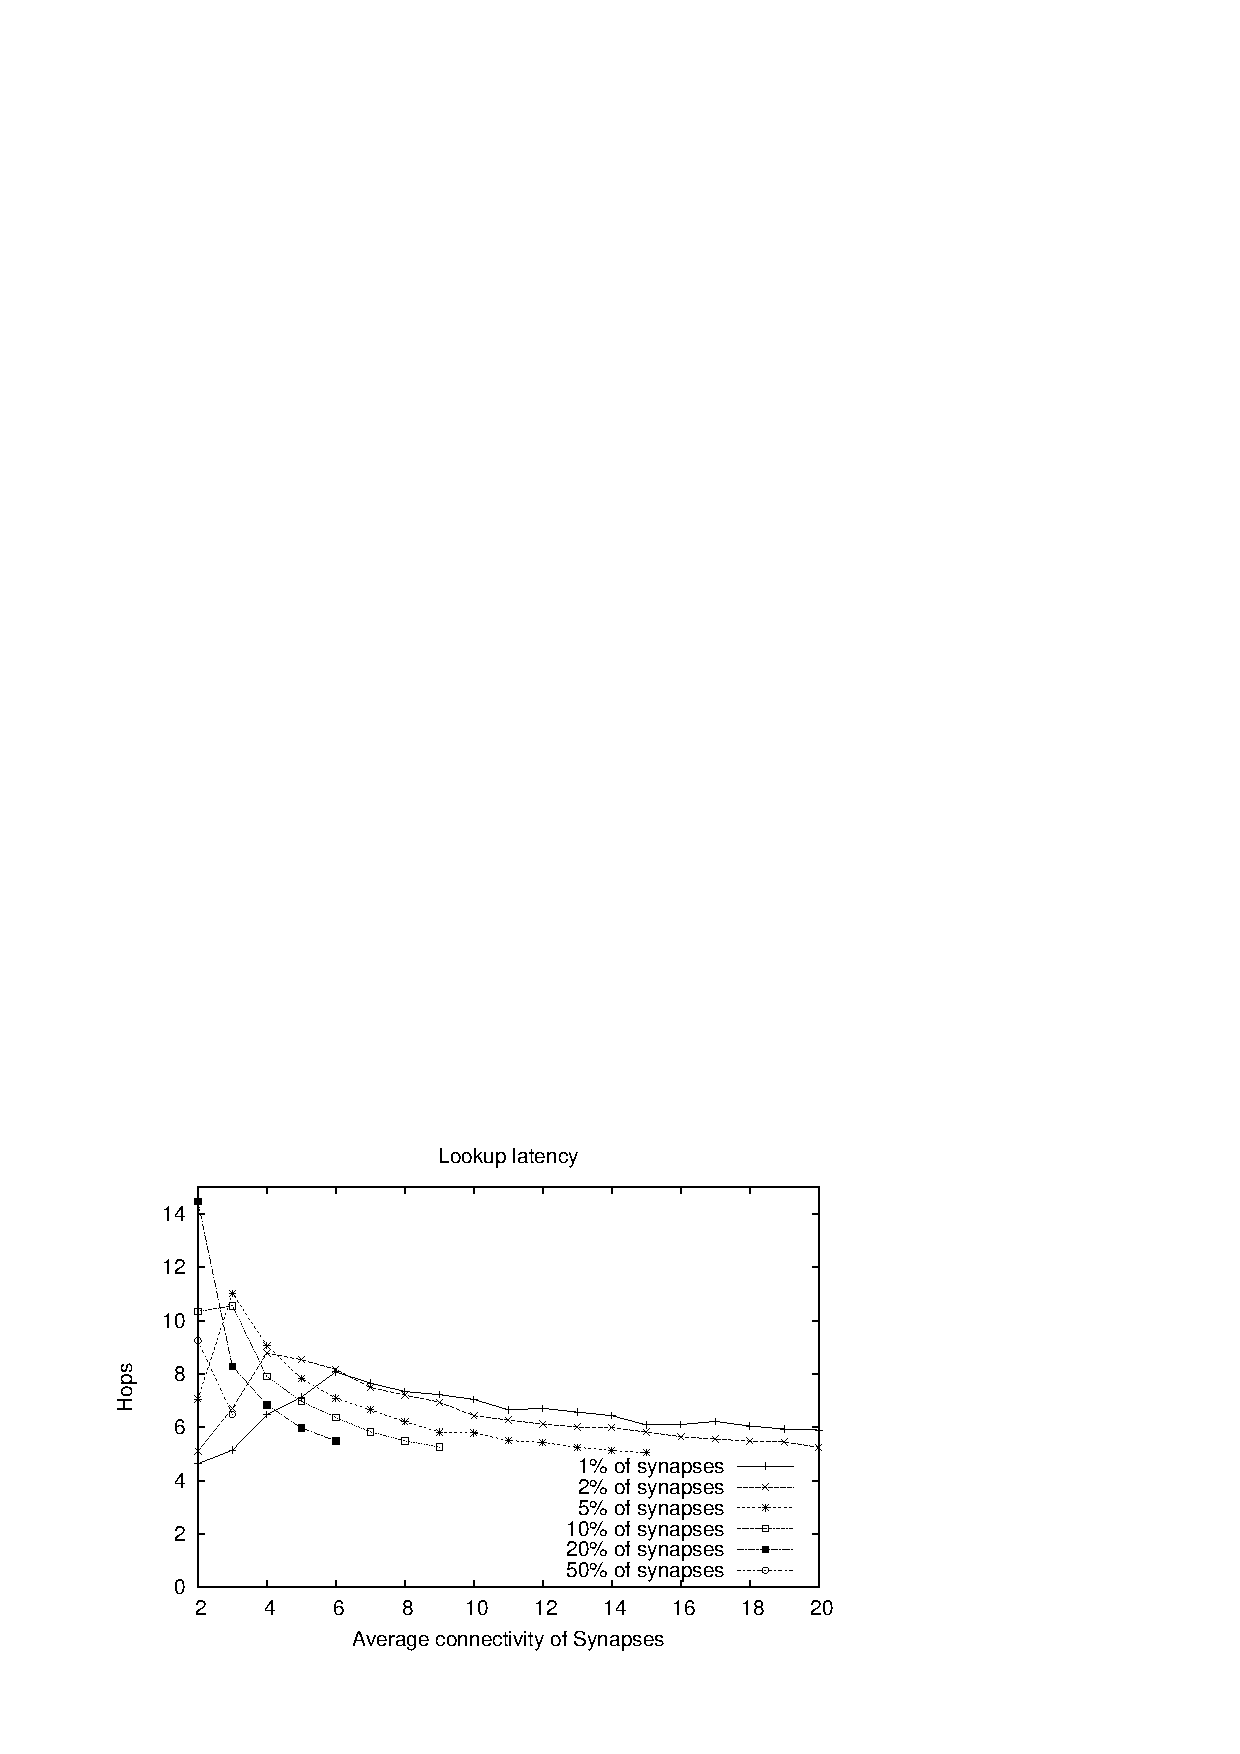
\includegraphics[width=\linewidth]{fig/3D-hops.pdf}
        \caption{Synapses and latency\label{fig:3D-hops}}
\end{figure}
%
Obviously, multiple searches in parallel lead to an increased number
of messages. As illustrated on Figure~\ref{fig:3D-msgs}, this number
can increases proportionally with the connectivity and number of
synapses. A good-deal strategy in synapses can leverage this
inter-network overhead.

% Moreover, the number of total communications tends to be linear in
% the number of nodes, which can obviously become a serious problem,
% as pointed out in unstructured networks.
%
\begin{figure}
        \includegraphics[width=\linewidth]{fig/3D-msgs.pdf}
        \caption{Synapses and communications\label{fig:3D-msgs}}
\end{figure}

%%% TTL simulations

\subsection{Time-To-Live}
%
We launched a second set of experiments in order to study the impact
of the TTL on the search queries. This TTL is simply decreased every
time the query traverses a node. The purpose is here to preserve a
significant exhaustiveness while reducing the amount of communications
undergone by the inter-overlay. We also made the number of overlays
vary, to experiment the impact of the \emph{granularity} of the
network. In other words, a Synapse network made of few large
structured intra-overlays could be called \emph{strongly structured},
and another network with many smaller structured intra-overlays could
be called \emph{weakly structured}. The number of nodes is still set
to $10000$, and every node is a synapse belonging to $2$ overlays
chosen uniformly at random.

Figure~\ref{fig:TTL-sat} confirms that this low connectivity ($2$) is
enough to achieve quasi-exhaustiveness. Another interesting result is
that TTL can be bounded without any impact on exhaustiveness ($10$ or
$12$ is enough even when the number of overlays interconnected is
$500$), while, as highlighted by Figure~\ref{fig:TTL-msgs}, drastically
reducing the amount of communications experienced, the number of
messages being almost divided by $2$.
%
\begin{figure}
        \includegraphics[width=\linewidth]{fig/TTL-sat.pdf}
        \caption{TTL and exhaustiveness\label{fig:TTL-sat}}
\end{figure}
%
\begin{figure}
        \includegraphics[width=\linewidth]{fig/TTL-msgs.pdf}
        \caption{TTL and communications\label{fig:TTL-msgs}}
\end{figure}
%
Finally, as can we can see on both Figures~\ref{fig:TTL-sat}
and~\ref{fig:TTL-msgs}, the \emph{granularity} does not significantly
influence exhaustiveness and communications when the number and
connectivity of the synapses are fixed.

\subsection{Peers' churn}
%
Since networks are intended to be deployed in dynamic settings (nodes
joining and leaving the network without giving notice), we conducted a
final set of simulations to see the tolerance of Synapse compared to a
single overlay network. Our simulations are again based on Chord. In
other words, the question is \emph{Would an interconnection of small
  Chords better tolerate transient failures than one large Chord?} In
this experiment, at each step, a subset of nodes is unreachable,
making message routing fail. As we can see on
Figure~\ref{fig:churn-sat}, a real improvement on the number of
satisfied requests can be obtained through a Synapse like network:
When the probability of failure at each step of a node increases, the
global availability of the network is far less reduced, making such
architecture more robust on the client's point of view and thus good
candidates for information\,retrieval\,on\,dynamic\,platforms.
%
\begin{figure}
        \includegraphics[width=\linewidth]{fig/churn-sat.pdf}
        \caption{Churn and exhaustiveness\label{fig:churn-sat}}
\end{figure}
